\documentclass[usenames,dvipsnames,10pt,aspectratio=169]{beamer} 

\usepackage[utf8]{inputenc}
\usepackage{verbatim}
\usepackage{minted}
\usepackage{graphicx}
\usepackage{wrapfig}
\usepackage{geometry}
\usepackage{listings}
\usepackage{color, xcolor}
\usepackage[document]{ragged2e}
\usetheme{umu}

\usemintedstyle{monokai}

\usepackage{hyperref}
\hypersetup{
    colorlinks=true,
    linkcolor=ucugreyish,
    filecolor=ucured,
    urlcolor=ucublue,
}
\urlstyle{same}

%%% Some useful commands
% pdf-friendly newline in links
\newcommand{\pdfnewline}{\texorpdfstring{\newline}{ }} 
% Fill the vertical space in a slide (to put text at the bottom)
\newcommand{\framefill}{\vskip0pt plus 1filll}

%%% Enter additional packages below (or above, I can't stop you)! / Jesper
\renewcommand{\proofname}{\sffamily{Proof}}

% presentation template slides usage
% \framecard[color (not working)]{textbuf}
% \framesplit{Header}{picture}{textbuf}
% \framepic{image}{text}

%%%%%%%%%%%%%%%%%%%%%%%%%%%%%%%%%%%%%%%%%%%%%%%%%%%%%%%%%%%%%%%%%%%%%%%%%%%%%%%%%%%%%
\title{Linux course}
\subtitle{Shell}
\date[\today]{\small\today}
\author[Morhunenko Mykola]{Morhunenko Mykola}
\institute{APPS@UCU}

\begin{document}

\begin{frame}
\titlepage
\end{frame}

\begin{frame}{\contentsname}
\setbeamercolor{background canvas}{bg=ucugrey}
\tableofcontents
\end{frame}

\section{What is Command Shell?}
\framepic{graphics/cli.jpg}{\bf{What is command shell?}}

\begin{frame}{Command Shell}
\begin{itemize}
    \item Command Shell is a computer program which provides user with a (CLI) command line interface to control the computer using keyboard, without GUI (Graphical user interface), for communication with the Linux system
    \item If you use Linux, you have definitely seen the command prompt. Usually it looks like {\color{ucugreen}\$} or, probably, {\color{ucugreen} \text{[username@hostname path] }\$}
    \item From the very beginning it looks like GUI is faster, but it is totally false: CLI just has high entry threshold. But it allows to write scripts (files with shell commands) that can automate routine, which is impossible in GUI
    \item Much more programs provide only CLI. If you want to use servers and connect to other computers via ssh, then being a real programmer is knowing shell
    \item You can check your shell by the command {\color{ucugreen} \$ echo \$SHELL}
    \item Most likely you have {\color{ucugreen} bash}, the most popular and stable one
    \item If you are done, you can exit shell with {\color{ucugreen} exit} command, or by pressing the {\color{ucugreen}Ctrl+d} in the terminal emulator window
\end{itemize}
\end{frame}

\begin{frame}{What is Bash}
\begin{itemize}
    \item Bash stands for "Bourne(born)-again-shell"
    \item It is the default shell for most Linux distros
    \item POSIX standard has a full description of shell. Bash implements all this features, plus something of its own, known as {\color{ucugreen} bashism}
    \item Bash is a standard shell for the majority of Linux distros, but it doesn't mean it is the best one
\end{itemize}
\end{frame}

\begin{frame}{ZSH}
    \begin{itemize}
        \item Zsh stands for {\color{ucugreen}Z-shell}
        \item Like Bash, it derives from Bourne family of shells, in everyday usage zsh is the same, as {\color{ucugreen} bash}, but has a lot of extensions and other configuration files' syntax (default - {\color{ucugreen} \textasciitilde/.zshrc})
        \item There is an entire eco-system of configuration tools and themes called oh-my-zsh which is very popular
        \item There is a huge amount of extensions on github, that can make everyday usage easier - ranging from auto-complete to syntax highlighting
        \item There are differences in scripts, we'll pick this up later.
        
    \end{itemize}
\end{frame}

\section{Paths}

{ % all template changes are local to this group.
    \setbeamertemplate{navigation symbols}{}
    \begin{frame}<article:0>[plain]
        \begin{tikzpicture}[remember picture,overlay]
            \node[at=(current page.center)] {
                
\includegraphics[keepaspectratio,width=\paperwidth]{graphics/path.jpg}
            };
        \end{tikzpicture}
     \end{frame}
}

\begin{frame}{Path}
    \begin{itemize}
        \item  {\color{ucugreen} Path} - one of the most important terms in this topic (and in understanding how programs work)
        \item Current path - or current directory, working directory - the directory, from where you are working, launching programs/scripts
        \item Paths can be absolute or relative
        \item Absolute
            \begin{itemize}
                \item {\color{ucugreen} /} - also known as  {\color{ucugreen} root path}, all paths that starts from it are {\color{ucugreen} absolute}. Other examples:
                \item {\color{ucugreen} /home/username}
                \item {\color{ucugreen} /usr/local/share/zsh/site-functions/}
            \end{itemize}
        \item Relative
            \begin{itemize}
                \item Relative paths don't start from the root. Shell interpreter always run all programs with respect to the current path. They never begin with \ex{/}
                \item {\color{ucugreen} .zshrc}
                \item {\color{ucugreen} Documents/UCULinux/presentations}
            \end{itemize}
    \end{itemize}
\end{frame}

\begin{frame}{Paths}
    \begin{itemize}
        \item Names are case-sensitive, which means {\color{ucugreen} /home/UserName} and {\color{ucugreen} /home/username} are different names
        \item There are also special paths
        \begin{itemize}
            \item {\color{ucugreen} ./} stands for the current path
            \item {\color{ucugreen} ../} stands for the path one step back. For example, if the {\color{ucugreen} ./} is {\color{ucugreen} /home/username}, the {\color{ucugreen} ../} will be {\color{ucugreen} /home}
            \item {\color{ucugreen} \textasciitilde /} stands for the directory of current user. For example, for {\color{ucugreen} root} user {\color{ucugreen} \textasciitilde/} will be {\color{ucugreen} /root}, and for {\color{ucugreen} username} it will be {\color{ucugreen} /home/username}
        \end{itemize}
    \end{itemize}
\end{frame}

\begin{frame}{PATH}
    \begin{itemize}
        \item 
    \end{itemize}
\end{frame}

\section{Bash Intro}
\framepic{graphics/bash.jpg}{Bash intro}

\begin{frame}{Syntax}
    All default commands (programs) have very similar syntax
    \begin{examples}
    \text{program\_name [option]... [arguments]...}
    \end{examples}
    Options starts from \ex{-} or \ex{-{}-} \newline
    To see, how to use any command
    \begin{examples}
        \text{program\_name -h} \newline or
        \text{program\_name -{}-}help \newline behind are synonyms, but parameters are in short and long forms \newline
        man \text{program\_name}  - it provides full documentation about the command
    \end{examples}
\end{frame}

\begin{frame}{Base commands}
\begin{itemize}
    \item \ex{pwd} - print working directory - show your current path
    \item \ex{ls <path>} - list - show what is inside the directory
    \item \ex{cd [path]} - change directory - change your current directory
\end{itemize}
Now it is possible to get something 
\begin{examples}
    username\$ pwd \newline
    \ex[ucugrey]{> /home/username} \newline
    username\$ ls \newline
    \ex[ucugrey]{> Desktop Documents Downloads Music Pictures Videos} \newline
    username\$ cd Downloads \newline
    username\$ pwd \newline
    \ex[ucugrey]{> /home/username/Downloads}
\end{examples}
\end{frame}
\begin{frame}{Base commands}

{\Large{Introducing ls}} \newline
\begin{itemize}
    \item \ex{ls -a} - list all, including names starting with the dot symbol "."
    \item \ex{ls -l} - list using a long list format, to display more information including permissions, size and important dates
    \item \ex{ls -r} - list in reversed order
    \item \ex{ls -R} - list current directory and all subdirectories recursively
    \item \ex{ls -S} - sort by file size, larger first. They can be combined as well.
\end{itemize}
The most commonly used are:
\begin{itemize}
    \item \ex{ls -la} - list all with full info. The command has path as an argument so the following command is also valid
    \item \ex{ls -la /etc/systemd/system}
\end{itemize}
There are much more options, that can be found using \ex{ls -{}-help}
\end{frame}

\begin{frame}{Base commands}
    Now it is possible to move around the directories and see, what is around. In order to work on labs or projects it's usually required to create something and see what is inside being able manipulate it somehow: \newline
    \begin{itemize}
        \item \ex{mkdir [dirname]} - make directory - create a new directory
        \item \ex{touch [filename]} - create a file with filename or update the date of file's last modification to the current date
        \item \ex{date} - print current date and time
        \item \ex{echo [text]} - print text to the standard output
        \item \ex{cat [filename]} - short for concatenate - show the file's content
        \item \ex{cp [source...] [destination]} - copy - copy all from source (all arguments except the last one) to the destination (the last argument). \ex{-r} option required for directories
        \item \ex{mv [source...] [destination]} - move - move all from source to destination
        \item \ex{rm [path]} - remove - remove the file. \ex{-rf} required for directories
    \end{itemize}
\end{frame}

\begin{frame}{Going deeper}

    {\Large Creating Links} \newline
    In Linux there are two types of links: hard and symbolic
    \begin{itemize}
        \item Inode - a data structure in the Unix-style file systems, that describes a file-system object
        \item Inode can have any number of hard links, and the inode will persists on the system until all hard links disappear. Changing in one file applies these changes also to all its hard links
    \end{itemize}
\end{frame}

\begin{frame}{Going deeper}
    \begin{itemize}
        \item \ex{ls -i} command is used to list all files with it's inodes
        \item \ex{ln [source] [destination]} is used to create hard links
        \begin{examples}
            username \$ ln file1 file2 \newline
            username \$ ls -i \newline
            \ex[ucugrey]{> 9700529 file1  9700529 file2}
        \end{examples}
        it is noticeable that both files have similar inodes
        \begin{examples}
        username \$ echo "Hello World!" >> file1 \newline
        username \$ cat file2 \newline
        \ex[ucugrey]{> Hello World!}
        \end{examples}
        Changes in one file apply these changes to the other one \newline
    \end{itemize}
\end{frame}

\begin{frame}{Going deeper}
    What about symbolic links?
    \begin{itemize}
        \item symbolic links (symlinks) are used more often. This is a special type, and the link refers to another file by name, not by inode.
        \item deleting the source file will make the symlink broken
        \item \ex{ln -s} - used to create the symbolic link
        \begin{examples}
        username \$ ln -s file1 file3 \newline
        username \$ ls -l \newline
        
        > -rw-rw-r-- 2 username groupname 18 Apr 17 00:47 file1 \newline
        \, \, -rw-rw-r-- 2 username groupname 18 Apr 17 00:47 file2 \newline
        \, \, lrwxrwxrwx 1 username groupname  5 Apr 17 00:54 file3 -> file1
        \end{examples}
        \item Symlinks can be created for any type of file system objects
        \item Can be used to point to an object from another file system
    \end{itemize}
\end{frame}

\begin{frame}{Going deeper}

    {\Large Wildcards, Globs}
    \begin{itemize}
        \item In case, there is a folder with 25 test files, but it is necessary to delete first 8 of them... there are few ways how to deal with that
        \begin{examples}
        username \$ rm test1 test2 test3 test4 test5 test6 test7 test8 \newline
        \,\,\,or... \newline
        username \$ rm test[1-8] \newline
        \,\,\,or if you want to delete all tests... \newline
        username \$ rm test*
        \end{examples}
        \item So, \ex{*} wildcard stands for all matches, any number of any symbol
        \item \ex{?} stands for \ex{any one symbol}
        \item \ex{[]} wildcard stands for ranges, so \ex{[abc]} means "any of a, b, c", the same for [a-c]
        \item \ex{!} stands for non-match, so [!a] stands for any symbol except 'a'
    \end{itemize}
\end{frame}

\begin{frame}{Going deeper}

    {\Large Important about wildcards}
    \begin{itemize}
        \item Be careful while using wildcards
        \item Bash preprocess all input to extend it with respect to wildcards
        \item so if you want to use one of such symbols just as symbols, you can either escape character with \ex{\textbackslash} symbol, or use single quotes
        \begin{examples}
        username \$ echo [fo]* > ./new\_file \newline in this case you will add names of all files starts with 'f' or 'o' \newline
        username \$ echo '[fo]*' > ./new\_file\newline
        username \$ echo \textbackslash [fo\textbackslash ]\textbackslash * > ./new\_file \newline
        both approaches above are correct
        \end{examples}
        \item \ex{ All bash commands are \href{https://ss64.com/bash/}{here}}
    \end{itemize}
\end{frame}

\begin{frame}{Searching}
    \begin{itemize}
        \item So as for now we know how to create files, directories, move them and remove. But how to find them?
        \item The Linux file system is well-structured, so it's very easy to navigate it, but still, there are thousands of files and it's impossible to remember all of the locations. There is entire presentation about the Linux File system hierarchy.
        \item \ex{find [path] -name ["filename"]}, and in the name can globs can be used (but they must be escaped)
        \item But if you don't know for sure the filename or dirname, the better way is \ex{find <path> -regex ["filename\_regex"]}
        \item \ex[ucured]{Be careful!} All files in the system have their own permissions. In order to search somewhere outside the \ex{/home/username} folder, you must run the program in the privileged mode
        
    \end{itemize}
\end{frame}

\begin{frame}[fragile]{Redirections}
    \begin{itemize}
        \item As it will be covered in the File systems overview lecture, one of the defining features of Unix is that everything is a file
        \item Even Shell is a group of files
        \item By default, in Unix systems programs read the input from a so called \ex{stdin} (input from the keyboard), write the output to the \ex{stdout} and write errors to the \ex{stderr}
        \item Redirections allows to change the input/output files
        \begin{itemize}
            \item \ex{0<filename or <filename} -- input from the \ex{filename}
            \item \ex{1>filename or >filename} -- output to the \ex{filename}, rewrite the file content
            \item \ex{1>>filename or >>filename} -- output to the \ex{filename}, add to the file content
            \item \ex{2>filename} -- error to \ex{filename}, rewrite the file content
            \item \ex{2>>filename} -- error to \ex{filename}, add to the file content
            \item \ex{\&>filename} -- both output and errors to \ex{filename}
            \item \ex{2>\&1} -- errors to \ex{stdout}
        \end{itemize}
    \end{itemize}
    \begin{lstlisting}[language=Bash, style=shellstyle]
    username $ ls >> some_file # No output to the 
    username $ cat some_file # show the content of some_file
    > Documents Downloads Music Pictures Programs \end{lstlisting}
\end{frame}

\begin{frame}[fragile]{Pipes}
    \begin{itemize}
        \item Sometimes it's required to give one program output of the other program (some kind of composition)
        \item There are pipes for such cases
        \item Pipe can be made by the \ex{|} symbol
        \item \ex{wc} - Word Count program, used to... count words (also letters, lines etc)
        \begin{lstlisting}[language=Bash, style=shellstyle] 
username $ ls -la | wc -l
> 23 
\end{lstlisting}
        \item That means that there are 23 lines of output
        \item Pipes are powerful, and one of must-know and must-use instruments
    \end{itemize}
\end{frame}

\begin{frame}{History}
    \begin{itemize}
        \item All shell commands are saved to the \ex{.bash\_history} or \ex{.zsh\_history}
        \item \ex[ucured]{If you want to make "anonymous" command (not store it to the history file) just start the command from the space}
        \item There are important environment variables:
        \item \ex{HISTSIZE} indicates how many commands from your history file are loaded into the shell's memory
        \item \ex{SAVEHIST} indicates how many commands your history file can hold
        \item \ex{All important variables are \href{https://telegra.ph/BashPeremennye-i-argumenty-09-19}{here}}
        \item \ex{ZSH} has special extensions for a better work with the history
        \begin{itemize}
            \item \ex{zsh-autosuggestions} -- suggests you the last command from the history 
            \item \ex{zsh-z} - \ex{cd} command alternative, but with some history analysis
        \end{itemize}
    \end{itemize}
\end{frame}

\begin{frame}{Hot keys}
    \begin{itemize}
        \item Usually people use only \ex{Ctrl + Shift + C, Ctrl + Shift + V, Ctrl + C, Ctrl + Z}, Though there are a lot of other useful hotkeys:
            \begin{itemize}
                \item \ex{Ctrl + n or arrow-up} -- next command in the history
                \item \ex{Ctrl + p or or arrow-down} -- previous command in the history
                \item \ex{Ctrl + c} -- SIGINT signal to the program (SIGnal INTerrupn, usually stops the process)
                \item \ex{Ctrl + l} -- clear the screen, call \ex{clear} program
                \item \ex{Ctrl + x; Ctrl + e} -- open the \ex{\$EDITOR} to change the inputted command; if there is no command, just open the \ex{\$EDITOR}
                \item \ex{Ctrl + z} -- freeze current program
                \item \ex{Ctrl + Shift + C} -- copy text to the global clipboard
                \item \ex{Ctrl + Shift + V} -- paste text from the global clipboard
                \item \ex{Tab} - completion/suggestions of the command
            \end{itemize}
        \item Full list available \href{https://telegra.ph/BashGoryachie-klavishi-09-17}{here}
    \end{itemize}
\end{frame}


\section{Permissions}
% https://cdn.lynda.com/course/797737/797737-637478818535472268-16x9.jpg
\framepic{graphics/permissions.jpg}{}

\framesplitc{Extensions}{graphics/ext.jpg}{
    \begin{itemize}
        \item The Linux world doesn't need file extensions
        \item The operating system doesn't use them to determine how to open a file
        \item But extensions are used by some parts of the OS to determine which program to use to open file
        \item How does the operating system find out, which is the file and how to deal with it?
    \end{itemize}
}

\begin{frame}[fragile]{Permissions}
    \begin{itemize}
        \item When executing the \ex{ls -l} command, at the very beginning of every line there is 10 characters and then two words
    \end{itemize}
    \begin{lstlisting}[language=bash, style=shellstyle]
username $ ls -la
> drwxrwxr-x 10 username groupname 4096 Apr 20 02:21 dir
  -rw-rw-r-- 10 username groupname 4096 Apr 20 02:21 textfile
  -rwxr-xr-x 10 username groupname 4096 Apr 20 02:21 binary_file
        \end{lstlisting}
    \begin{itemize}    
        \item They are not just letters, there is a lot of information behind these 10 characters (or, actually, 3 decimal numbers)
    \end{itemize}
\end{frame}

\begin{frame}{Permissions}
    \begin{figure}
        \centering
        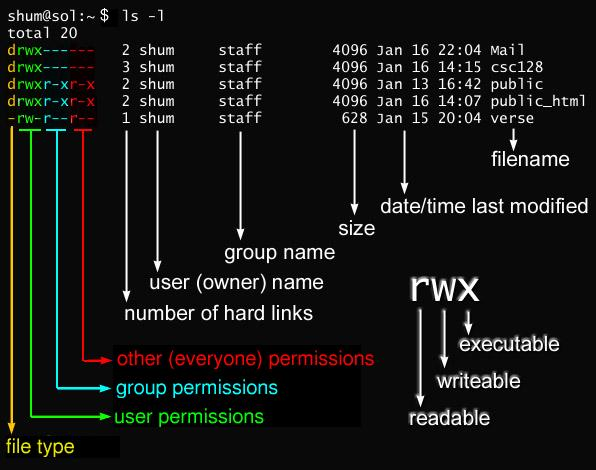
\includegraphics[height=0.8\paperheight]{graphics/permissions1.jpg}
\end{figure}
\end{frame}

\framesplitc{Permissions}{graphics/permissions.png}{
    \begin{itemize}
        \item The very first letter stands for the file type (this topic will be covered in the File systems presentation)
        \item To change permissions, there is a command \ex{chmod}
        \item To see all possible parameters, use \ex{chmod -{}-help}. (But some explanations for the beginners are on the next page)
        \item All triplets of permissions \ex{rwx} have theirs number correspondences
    \end{itemize}
}

\begin{frame}{Permissions}
    \begin{itemize}
        \item The outputoutput of \ex{chmod -{}-help}  may have some confusing stuff in it
        \item In \ex{[ugoa]} - User, Group, Other users, All
        \item In \ex{[rwxXst]} - Read, Write, eXecute
        \item eXecute only if the file is a directory or already has execute permission for some user
        \item Set user or group ID on execution
        \item Save program text on swap device (a performance enhancer)
    \end{itemize}
\end{frame}
% https://i.pinimg.com/originals/7c/cb/0e/7ccb0ef4eb7d6038c13dd7314ab61fb6.jpg
\framepic{graphics/sudo.jpg}{}

\framesplitc{Sudo}{graphics/sudo_meme.jpg}{
    \begin{itemize}
        \item By default, every user have permissions to play around only his \ex{/home/username} directory
        \item To somehow modify the system (either install programs or modify global settings), you need a so called \ex{superuser mode}
        \item If there's an error starting with \ex[ucured]{permission denied}, then it's necessary to run the program with privileges, for example, using \ex{sudo}
    \end{itemize}
}

\framesplitc{Sudo}{graphics/password_meme.jpg}{
    \begin{itemize}
        \item To run any program as a superuser, use \ex{sudo <program\_name> <program\_parameters>}, where sudo stands for "super user do"
        \item To login into the shall as a superuser, both \ex{su root} and \ex{sudo -i} can be used. \ex[ucured]{When you type a password, it stays invisible}
        \item \ex[ucured]{\large DO NOT RUN GUI AS ROOT!} instead use \ex{gksu} (it is deprecated for as 2021, but still in AUR) or alternatives (\ex{kdesu, sux})
    \end{itemize}
}

\begin{frame}[fragile]{Process Control}
    \begin{itemize}
        \item To stop the process use \ex{Ctrl + z} keybinding
        \item To unstop the process \ex{fg} program is used (foreground)
        \item To unstop the program but leave it in the background, \ex{bg} program is used (background)
        \item If you want some program to run at the background, \ex{\&} symbol is used
        \begin{lstlisting}[language=bash, style=shellstyle]
username $ clion &
> [1] 117306 \end{lstlisting}
        \item This command will start a \ex{clion} from the current environment, but the command line still will be available for the input
        \item \ex[ucured]{Be careful.} After such command all clion output will still be printed to the stdout (if not redirect it)
        \item \ex{jobs -l} -- list all background jobs
    \end{itemize}
\end{frame}

\begin{frame}[fragile]{Process Control}
    \begin{itemize}
        \item Signals - one of possible ways how different processes communicate with each other in the POSIX systems
        \item To sent signal to the process ID (that 5-6 digits numbers) \ex{kill} command can be used
        \item \ex{SIGTERM} - kill sends it by default, which means stopping the program (TERMinate)
        \item \ex{SIGINT} - Interrupt the process, the hotkey is \ex{Ctrl + C}
        \item But \ex{jobs} program shows only processes started from the current session
        \item \ex{ps} program used to see all processes, their PIDs and other info
        \begin{lstlisting}[language=bash, style=shellstyle]
username $ ps ax
> PID TTY      STAT   TIME COMMAND
    1 ?        Ss     0:02 /sbin/init     
    2 ?        S      0:00 [kthreadd]
    3 ?        I<     0:00 [rcu_gp]
    .....\end{lstlisting}
        \item So to stop the process immediately, just run \ex{kill [PID]}
    \end{itemize}
    
\end{frame}

\section{Scripts}
% redirections, variables etc.
\framecard{Scripts}

\begin{frame}[fragile]{Scripts}
    \begin{itemize}
        \item Script - just file with bunch of commands that can be interpreted (e.g. python, lisp scripts, or bash scripts)
        \item They can be used both for automation some small routine tasks and as large programs
        \item Shell scripts names ends with \ex{.bash}, \ex{.sh}, \ex{zsh}
        \item But as far as we know, the Linux system doesn't use the extensions to identify the type of the file. How to run a script as a usual program?
        \item One of possible ways to run the script is to give it as a parameter to the command interpreter
        \begin{lstlisting}[language=bash, style=shellstyle]
username $ bash ./my_first_script.sh
> some output
        \end{lstlisting}
    \end{itemize}
\end{frame}

\begin{frame}[fragile]{Scripts}
    \begin{itemize}
        \item Or make the file executable (add \ex{x} or \ex{111} flag)
        \begin{lstlisting}[language=bash, style=shellstyle]
username $ chmod +x ./my_first_script
username $ ./my_fist_script
> some output
        \end{lstlisting}
        \item Actually, there is a mistake. If you do it in the following way, the script will be run from the running shell. But we want to make Python, Ruby. Scheme also executable. Unfortunately, the bash interpreter can not execute them...
    \end{itemize}
\end{frame}

\begin{frame}{Shebang}
    \begin{itemize}
        \item \ex{\large Shebang} - the name of the character sequence at the very first line of the script (\ex[ucured]{line \#1, that is important!}) which specifies the absolute path to the interpreter.
        \lstinputlisting[language=Bash, style=codestyle]{code/shebang_ex.sh}
        \item Or also possible variant (to search for the interpreter in PATH (about PATH in next presentation))
        \lstinputlisting[language=Python, style=codestyle]{code/shebang_ex.py}
    \end{itemize}
\end{frame}

\begin{frame}[fragile]{Variables}
    \begin{itemize}
        \item  User can define and use variables at the environment:
        \begin{lstlisting}[language=Bash, style=shellstyle]
username $ my_var="This is my var"
        \end{lstlisting}
        \item \ex[ucured]{There is no space allowed on either side of the "=" sign}
        \item There are local and global variables
        \item When we "export" the var, it becomes available in all applications run from the current session, which means global 
        \item For programs running from the shell, global variables are the same as environment variables
        \item To get the variable, \$\{\} syntax is used:
        \begin{lstlisting}[language=Bash, style=shellstyle]
username $ echo ${my_var}
> This is my var
        \end{lstlisting}
    \end{itemize}
\end{frame}

\begin{frame}{Script arguments}
    \begin{itemize}
        \item Scripts (actually, all programs) are useless without some input from the user
        \item Just to remember, the default program calling syntax:
        \begin{examples}
            \text{program\_name [option]... [arguments]...}
        \end{examples}
        \item So to access the arguments:
        \begin{itemize}
            \item \ex{\$\{@\}} - all arguments
            \item \ex{\$\{\#\}} - number (length) of all arguments
            \item \ex{\$\{0\}} - script name
            \item \ex{\$\{1\}}, \ex{\$\{2\}}... - other script parameters
        \end{itemize}
    \end{itemize}
\end{frame}

\begin{frame}[fragile]{Quoting}
    \begin{itemize}
        \item As far as there are a lot of special characters, how to use them if you want to print them?
        \item Quoting or escaping is used to make a regular symbol from a special one
        \item \ex{\textbackslash} is used in a lot of programming languages
        \begin{lstlisting}[language=Bash, style=shellstyle]
username $ echo \$SHELL
> $SHELL
username $ echo ${SHELL}
> /bin/zsh \end{lstlisting}
        \item \ex{'} - single quotes, make "escaped" everything inside
        \item \ex{"} - double quotes, allow variables expansion
    \end{itemize}
\end{frame}

\begin{frame}{Conditionals. If}
    \begin{itemize}
        \item The standard \ex{if} with both one and many branches
        \lstinputlisting[language=Bash, style=codestyle]{code/if_syntax.sh}
        \item Example:
        \lstinputlisting[language=Bash, style=codestyle]{code/conditions_ex.sh}
    \end{itemize}
\end{frame}

\begin{frame}{Conditionals}
    \begin{itemize}
        \item There are a lot of conditions regarding different types:
        \item For numbers:
        \begin{itemize}
            \item \ex{-lt} - <
            \item \ex{-gt} - >
            \item \ex{-le} - <=
            \item \ex{-ge} - >=
            \item \ex{-eq} - ==
            \item \ex{-ne} - !=
        \end{itemize}
        \item Logical operations
        \begin{itemize}
            \item \ex{-a} - and
            \item \ex{-o} - and
            \item \ex{!} - not
        \end{itemize}
    \end{itemize}
\end{frame}

\begin{frame}{Conditionals}
    \begin{itemize}
        \item \ex{[-d FILE]} - True if FILE exists and is a directory
        \item \ex{[-e FILE]} - True if FILE exists
        \item \ex{[-f FILE]} - True if FILE exists and is a regular file
        \item \ex{[-r FILE]} - True if FILE exists and is readable
        \item \ex{[-s FILE]} -  True if FILE exists and has a size greater than zero
        \item \ex{[-w FILE]} - True if FILE exists and is writable.
        \item \ex{[-x FILE]} -  True if FILE exists and is executable
        \item \ex{[-z STRING]} - True of the length if ”STRING” is zero
        \item \ex{[-n STRING]} - True if the length of ”STRING” is non-zero
        \item For strings the most popular cooperators are used
        \item \ex{[[ ]STRING1 == STRING2 ]]} 
        \item the same about <, >, !=, etc
    \end{itemize}
\end{frame}

\begin{frame}{Conditionals. Case}
    \begin{itemize}
        \item If you have an experience in other programming languages, you should definitely know the case statement. Here is the example:
        \lstinputlisting[language=Bash, style=codestyle]{code/case_ex.sh}
    \end{itemize}
\end{frame}

\begin{frame}{Loops}
    If you know any programming language, you definitely know, what loop is. Here is bash syntax for them
    \lstinputlisting[language=Bash, style=codestyle]{code/for_syntax.sh}
    \lstinputlisting[language=Bash, style=codestyle]{code/while_syntax.sh}
    \lstinputlisting[language=Bash, style=codestyle]{code/until_syntax.sh}
\end{frame}

\begin{frame}{Loop examples}
    \lstinputlisting[language=Bash, style=codestyle]{code/for_ex.sh}
    \lstinputlisting[language=Bash, style=codestyle]{code/while_ex.sh}
\end{frame}

\begin{frame}{More \ex{for loop} examples}
    \lstinputlisting[language=Bash, style=codestyle]{code/for_extended_ex.sh}
\end{frame}

\begin{frame}[fragile]{Arithmetic}
    \begin{itemize}
        \item In bash arithmetic is a little bit tricky
        \item To evaluate the arithmetic expression, \ex{let} can be used
        \begin{lstlisting}[language=Bash, style=shellstyle]
username $ a=4+5
username $ echo $a
> 4+5
username $ a=((4+5))
username $ echo $a
> 9 \end{lstlisting}
        \item \ex{+, -, *, /, ** (power), \%, ++, --} commands can be used 
    \end{itemize}
\end{frame}

\begin{frame}[fragile]{Arrays}
    \begin{itemize}
        \item As all other programming languages, Bash has arrays
        \item Here is the syntax of using and introduction of the arrays (in ZSH it is a little different)
        \lstinputlisting[language=Bash, style=codestyle]{code/arrays_syntax.sh}
        \begin{lstlisting}[language=Bash, style=shellstyle]
username $ ./script.sh
> Apple Lemon Milk
        \end{lstlisting}
    \end{itemize}
\end{frame}

\begin{frame}[fragile]{Arrays}
    \begin{itemize}
        \item There are a lot of ways how to iterate through the array and other more important commands
        \lstinputlisting[language=Bash, style=codestyle]{code/arrays_iter.sh}
        \item Full list can be found \href{https://devhints.io/bash#arrays}{here}
    \end{itemize}
\end{frame}

\begin{frame}[fragile]{Functions}
    \begin{itemize}
        \item Function declarations can be like this:
        \lstinputlisting[language=Bash, style=codestyle]{code/function_ex.sh}
    \end{itemize}
\end{frame}

\begin{frame}[fragile]{Namespace}
    \begin{itemize}
        \item For example in C, the local variable (defined inside some scope) life cycle ends with the end of the scope
        \item On the opposite in Bash all declared variables overwrite the global one with the same names
        \item to prevent this, use \ex{local} definitions
        \lstinputlisting[language=Bash, style=codestyle]{code/namespace_ex.sh}
        \begin{lstlisting}[language=Bash, style=shellstyle]
username $ ./start.sh
> one two three 
  global hello\end{lstlisting}
    \end{itemize}
\end{frame}

\section{Sources}
\framecard{Sources}
\begin{frame}{Sources}
\begin{itemize}
    \item \href{https://cms.ucu.edu.ua/pluginfile.php/181565/mod_resource/content/3/os_p01_bash.pdf}{Bash presentation for Operating systems course, UCU, Oleg Farenyuk (only from UCU domain)}
    \item \href{https://www.funtoo.org/Linux_Fundamentals,_Part_1}{Linux basics from the founder of Gentoo, Daniel Robbins, Chris Houser, Aron Griffis}
    \item \href{https://www.funtoo.org/Bash_by_Example,_Part_1}{Bash basics, Daniel Robbins, Chris Houser, Aron Griffis}
    \item \href {https://scriptingosx.com/}{Scripting OS X}
\end{itemize}    
\end{frame}

\end{document}
